\chapter{State of the Art} \label{ch:pcreg}
The main subject of this paper is to register two or more point clouds. The goal of registration is to find the rigid transformation(s) that puts the point clouds in one common coordinate system. Applying this transformation will make surfaces of the object that occur in both overlap. The term ``alignment'' is often used interchangeably with ``registration'', though the former emphasizes that \emph{surfaces} are being aligned.

For registration to be meaningful, the hypothesis is made that the point clouds do represent scans of the same object, and that the \emph{true} rigid transformation(s) that align them exists. For the case of two 3D scans of a stationary object, this true transformation would be the camera pose of the first scan relative to that of the second scan. The goal of registration algorithms is then to find an estimation of the true transformation. Except for artificially generated testing data, the true transformation is usually unknown or known only at a limited precision.

This chapter consists of a classification and survey of existing registration methods.

\section{Point cloud registration}

\emph{Pair-wise} registration algorithms take one \emph{fixed} point cloud $P$ and one \emph{loose} point cloud $Q$ as input. The output is a rigid transformation $\emph{M}$ that brings $Q$ into the coordinate system of $P$. During the algorithm $P$ is left unchanged, while $Q$ gets moved around. Thus implementations can preprocess $P$ once to allow for more efficient computation, for example by representing it in a KdTree, so that closest points can be computed more quickly. The representation of $Q$ on the other hand may be modified on the fly, for example by applying a partial transformation to the points' coordinates after each iteration of the algorithm.

When the goal is to register multiple point clouds $\{ P_i \}$, a pair-wise algorithm could be applied multiple times to different pairs $(P_i, P_j)$. Depending on how these pairs are chosen, this leads to an asymmetric accumulation of the registration error. \emph{Multi-view} registration algorithms instead directly operate on a set of point clouds to align, and evenly distribute the registration error. The output is a set of rigid transformations $\{ \matr{M_i} \}$, one for each input point cloud. (If one point cloud $P_f$ is chosen as fixed, then $\matr{M_f} = \matr{I}$)

A primary distinction is made depending on whether an initial estimation for $\matr{M}$ is already known. This may come for example from manual alignment made in a 3D visualizer application, or from sensors attached to the scanners that detect its pose. \emph{Coarse registration} algorithms make no such assumption and use a representation of the point cloud that is invariant to its current pose relative to the other one, to deduce an approximate alignment. \emph{Fine registration} algorithms assume that the point clouds are already approximatively registered, and improve upon the alignment by bringing corresponding parts closer together. The goal is to obtain the most accurate solution possible. Some methods can also yield a fine registration, without initial registration.

In the most usual case the point clouds to register already have the same scale, so $\matr{M}$ is a proper rigid transformation. When this is not the case, for example when one of the point clouds was taken using photogrammetry and the real scale is unknown, the goal would additionally be to find a scaling factor. $\matr{M}$ would then be a composition of a proper rigid transformation followed by a scaling transformation.

There is also the notion of \emph{non-rigid registration}, which is a generalization where the loose point clouds can also be deformed. The output is no longer a single transformation matrix. Depending on the deformation model used, it may instead be for example a per-point displacement field, or a rigid transformation combined with a modification of a skeleton that parametrizes the deformation. It is used to register point clouds depicting one same object that can change shape in some limited way between the scans, for instance a waving flag, a human face or in medical imaging an internal organ. In this paper only rigid registration is considered.

Good surveys of existing registration methods are presented in \cite{Salv2006}, \cite{Tam2007} and \cite{Bell2014}.


\section{Robustness} \label{sec:registration_robostness}
The ideal case for registration of two point clouds $P$ and $Q$ would be if $P = \{ \matr{M} \, p : p \in P \}$, that is they both contain exactly the same constellation of points, with $Q$ being transformed by precisely the \emph{true} rigid transformation $\matr{M}$. Here $\matr{M}$ is the one unique (unless the model has precise rotation symmetry) rigid transformation which makes $P$ and $Q$ coincide, and it is possible for a trivial algorithm to compute $\matr{M}$ at an arbitrary level of precision, taking only $P$ and $Q$ as input.

However in practice $P$ and $Q$ will differ in many more ways than the rigid transformation. A registration algorithm is deemed to be \emph{robust} if it continues to deliver good results when the disparities between the point clouds get progressively worse.

These disparities can for example be the following:
\begin{description}
\item[Points dispersion] The points of a point cloud constitute a discrete subset of the surfaces. Unless $P$ and $Q$ were algorithmically generated from the same scanner output file, those subsets will be different but still represent the same surface. The lower the point density, the stronger this disparity becomes.

Points on a planar surfaces will typically be dispersed approximatively on a quadrilateral grid, when scanned using a laser scanner that proceeds in sequential scan-lines. It becomes a square grid on surfaces facing the scanner. The more the surface is oblique, the wider the lattice gets and the density gets lower.

When large objects are scanned, the points density will get lower on surface locations further away from the scanner. 

\item[Noise] One or both point clouds can contain outlier points that do not lie on any relevant surface of the model. They result from points that were scanned from the environment but are not part of the model surfaces, scanner errors, or artifacts from prior processing.

A good registration algorithm should be insensitive to outlier points, or be able to identify them and sort them out before continuing. The \emph{noise-to-signal} ratio can be defined as the number of outlier points divided by the number of inlier points.

\item[Bounds] The two point clouds contain only points within given geometric bounds, either due to the limited range and field of view of the scanner, or from having been cropped out of a larger point cloud in preprocessing.

While a minimal bounding box, frustum, etc. can be computed from a point cloud such that all its points are within it, the actual bounding region of the scan is usually not known. That is, if there is no point in a particular location, it is not immediately known whether this is because there is no object surface at that location, or because the location is out of bounds. (For range images, the field of view is known.)

But all points that are not within the intersection of these bounding regions of $P$ and $Q$ will have no corresponding point in the other point cloud, and so they need to be treated by the registration algorithm the same way as outliers.

\item[Occlusion] The scanner can only record surface points that are visible from its pose. Occluded areas will not be covered by the point cloud. Because no surface connectivity information is recorded, and sometimes the scanner position in the point cloud coordinate system is unknown, it becomes hard to tell what regions are occluded. Moreover because the surfaces are only partially covered, reconstructing them becomes a harder problem.

When registering two scans taken from different poses, their region of overlap becomes limited to the areas that are not occluded in either point cloud. Point outside it will have not corresponding point in the other cloud. But they still hold information about the underlying surface that is represented by both $P$ and $Q$.
\end{description} 


\section{Coarse Registration}
For coarse registration, no initial alignment of the point clouds is used, and the goal is to obtain an approximative alignment, which can then be improved upon using fine registration.

Coarse registration algorithms typically do not look at the point cloud in detail, but rather at some larger scale descriptor of its shape. They are used to roughly align entire scans that have outliers, relatively small overlap and many complex features that would need more prior filtering to work with fine registration algorithms.

\subsection{Manual registration}
Most commonly, coarse registration is done manually. One method is to define at least three pairs of corresponding positions in the two point clouds, another is to rotate and translate the point clouds using a 3D interface.

Both methods can be time consuming, because one works using a two-dimensional projection of the two point clouds on a computer screen, the view is difficult to recognize when they overlap incorrectly, and one needs to be able to rotate and translate both the camera, and the two point clouds. For these reasons automatic solutions may be preferred in practice, especially when the scanning project consists of many point clouds.

In the context of robotics, or when mobile scanners are being used, an estimation for the scanner poses, and with it of the point cloud alignment is often recorded using odometric sensors.


\subsection{Feature correspondence}
Instead of manually specifying corresponding positions, the process can be automated by placing visual markers on the scene prior to scanning. These can be detected automatically and used to get a rough estimation of the scanner pose. \cite{Mati2011} describes one procedure where two-dimensional visual markers are used.

It is also possible to use image analysis to find corresponding features on two photographs that have been registered to the scans, and register the point clouds based on those. \cite{Tour2009} Here image feature detection can be used, in particular invariant (to rotation and scaling) descriptors such as SIFT or SURF. An extensive survey of feature detectors is given in \cite{Tuyt2007} and \cite{Saxe2014}.

It is also possible to identify and put into correspondence features such as lines \cite{Lich2011}, planes \cite{Dold2006} or NURBS curves \cite{Koch2008}.


\subsection{Extended Gaussian Image}
The \gls{egi} is one descriptor of the entire point cloud that can be used to estimate a rough rotational alignment. Planar surfaces are identified in the point clouds $P$ and $Q$ and their normal vectors are recorded. \cite{Dold2005} From this a kind of spherical histogram of the normal vectors is constructed. When $P$ and $Q$ represent the same object with enough overlap, these histograms will have a similar shape, but be rotated differently.

A normal vector can be described using two spherical coordinates $\theta, \phi$. The \gls{egi} is defined as the projection of the set of normal vectors onto the unit sphere. \cite{Horn1984} Information about the positions of the planes whose normal vectors were taken is lost.

Because of the topology of the sphere surface, there is some difficulty in representing the \gls{egi} digitally. Unlike a planar surface like a rectangular image, it cannot easily be divided into ``pixel'' cells of equal area. The surface should ideally be divided into cells in such a way that (1) all cells have approximatively the same area and shape, (2) they must be small enough, and (3) some rotations will make cells (approximatively) coincide.

A division along longitude and latitude axis does not meet the first and third constraints. Platonic solids have equal area cells but are limited to $20$ triangular faces. A good compromise is the so-called \emph{geodesic division}.

The \gls{egi} is represented by storing for each of these cells the number of normal vectors that fall into it. To find an approximate rotational alignment, the \gls{egi}s of $P$ and $Q$ are normalized, and then the \gls{egi} of $Q$ is rotated for all spherical angles $\theta, \phi$. A measure of how well the \gls{egi}s match is taken. This may for instance be the sum of squared or absolute differences of the values of coinciding cells, or their correlation. The estimated rotational registration is then given by the angles for which this metric is maximized.

An extension which is more stable to low overlap and which includes the estimation of a translation is described in \cite{Maka2006}.


\section{Fine registration}
Fine registration algorithms take as input two (or more) point clouds that are already approximatively aligned, and then improve this alignment as much as possible. The core observation is that corresponding points in the two point clouds are already close to each other with the current alignment.

\subsection{Iterative Closest Point} \label{sec:icp}
The most well-known fine registration algorithm is \gls{icp}, first described in \cite{Besl1992} and in \cite{Chen1991}. It is a pair-wise algorithm, though multi-view versions of it also are also possible \cite{Told2010}.

The algorithm chooses \emph{point correspondences} $(p \in P, q \in Q)$, where $q$ is the point closest to $p$ with the current alignment. Using the assumption that $P$ and $Q$ are already roughly aligned, those correspondences approximatively correspond to real corresponding point in both representations of the object. Then a rigid transformation is applied to $Q$ which minimizes the distances $d(p, q)$ for all corresponding point pairs in a least squares sense. The process is repeated iteratively.

Different terms for the fixed and loose point clouds are frequently used in the literature. For example the fixed point cloud may be called ``model'', ``target'' or ``reference''. The loose one may be called ``data'' or ``source''. In this text the terms ``fixed'' and ``loose'' are used.

\subsubsection{ICP framework}
There are many possible variations of \gls{icp} algorithms \cite{Rusi2001}. For all of them the following six steps are performed at each iteration:
\begin{description}
\item[Selection] Select a subset of points from $P$ and/or $Q$ to consider. In the simplest case all points are considered. Alternatives include the selection of a random subset with a given down-sampling ratio. The decision to include or reject a point, or the probability of including a given point, may depend on a given metric, such as its distance to the center, distance to the closest neighbour, orientation of normal vector, and others. Here the selected subsets are called $P^*$ and $Q^*$ respectively.
\item[Correspondence] Build correspondence pairs $(p_i, q_i)$ using the selected points. The \emph{closest point criterion} is to choose for each $p \in P^*$ the point $q \in Q^*$ (or the other way) whose Euclidian distance $\|p - q\|$ to it is minimal. Here $p_i$ and $q_j$ denote corresponding points when $i = j$. It is not necessarily a one-to-one mapping: A point from one cloud may correspond to multiple point from the other.

There are other strategies for choosing point correspondences. When the normal vectors $\vec{n_p}$ are known, one possibility is to choose $q \in Q^*$ that is closest to the ray pointing out of $p$ in the direction of its normal vector $\vec{n_p}$. Also it can be useful to only consider points in $Q^*$ that satisfy certain constraints in function of $p$, such as a similar normal vector orientation, color, or other.

It is also not necessary for both $P$ and $Q$ to be point clouds. For example $Q$ may instead be defined using a parametric surface, such as the set of triangles forming a mesh. For each $q$ a corresponding point $q'$ is then computed from $p$, instead of being chosen from a fixed finite set.

Finding correspondences is typically the most computationally intensive operation in the \gls{icp} iterations. One way to optimize closest point finding it is to use an appropriate data structure for $Q$, for example a KdTree. Also if $Q$ is available as a range image with known camera parameters, $p$ can be projected onto the 2D range image. Then the search can be limited to a certain radius surrounding the projection of $p$ in image space.
\item[Rejection] Some correspondence pairs may be rejected afterwards. For example those where the distance is above a certain threshold value.
\item[Weighting] Optionally weights may be associated with the correspondences. Unless the correspondences perfectly match real corresponding points in both clouds, a rigid transformation that makes $P^*$ and $Q^*$ coincide is impossible. Defining weights introduces a bias in the distribution of the remaining error: The transformation will move correspondences with higher weight closer together than those of lower weight.

Commonly correspondences where the distance $\| p - q \|$ is higher get attributes a lower weight. The weights may also be set to compensate for surface areas where the density of points $q$ is lower. Alternatively, correspondences attributes with a lower confidence value may get a lower weight.
\item[Error estimation] An expression of the registration error $e(\matr{M})$ in function of the correspondences $\{ (p, q) \}$ and the rigid transformation $\matr{M}$. $e(\matr{M}) = 0$ when $P^*$ and $\matr{M} \, Q^*$ perfectly coincide. This value can only be reached in theoretical settings where the correspondence pairs have been set to be equal to real corresponding points on the object.

The algorithm will compute the transformation $\argmin_{\matr{M}} e(\matr{M})$ that minimizes the error. When $e(\matr{M})$ is below a predefined threshold value, the algorithm stops and the registration is considered successful. A common problem is that $e(\matr{M})$ may have local minima, which can lead the algorithm to converge towards an incorrect registration. 

For \emph{point-to-point} \gls{icp}, the weighted sum of squared Euclidian distances of corresponding points is used:
$$
e(\matr{M}) = \frac{1}{W} \sum_{i} w_i \, \| p_i - \matr{M} \, q_i \|^2
$$
where $W = \sum_i w_i$. For \emph{point-to-plane} ICP, instead the distances from $q$ to the tangent plane of $p$ are used. This requires knowledge of the normal vectors $\vec{n_p}$ associated with the points $p$. It is computed using the dot product of $\vec{n_p}$ and $\vec{p} - \vec{q}$:
$$
e(\matr{M}) = \frac{1}{W} \sum_{i} w_i \, \vec{n_{p_i}} \n (p_i - \matr{M} \, q_i)
$$
Intuitively, with this metric, $e(\matr{M})$ remains unchanged when two parallel surfaces ``slide'' along each other. With point-to-point, the different distributions of points on the two surfaces can lead to local minima. Point-to-plane typically increases convergence speed and robustness, but is more computationally expensive.

Several other error metrics to minimize have been developed, such as Generalized ICP \cite{Sega2009}, Sparse ICP \cite{Boua2013}, and metrics that include attributes of the points such as its color value.

\item[Minimization] The $\matr{M}$ for which $e(\matr{M})$ is minimal is computed. For the point-to-point error metric it is a least squares problem, and a closed-form solution is possible as detailed in section \ref{sec:lsq_align}. A comparison of four methods is made in \cite{Loru1995}. It is concluded that the difference between the different methods are small.

For the point-to-plane metric, a similar solution is also possible by linearizing the problem using the small-angle approximation of trigonometric functions. \cite{Chen1991} For this the assumption is made that incremental rotations are small, which hold when the point clouds start out approximately aligned and converge to their optimal alignment.

There are also extrapolation methods that make an estimation of $\matr{M}$ based on previous iterations in order to improve efficiency, and methods that introduce randomisation to avoid convergence to a local minimum. \cite{Rusi2001}
\end{description}

Any iterative algorithm that follows these steps is said to be in the \emph{ICP framework}. The original description \cite{Besl1992} of \gls{icp} selects correspondences using the closest-point-criterion, and applies a point-to-point error metric. \cite{Chen1991} describes a point-to-plane variant.


\subsubsection{Convergence}
\gls{icp} is based on estimating correspondences for the points of $P$ in $Q$. If the best possible correspondences were known to start with, point cloud alignment could be solved in one iteration using a least-squares solution as described in \ref{sec:lsq_align}. \gls{icp} instead uses the fact that $P$ and $Q$ are already approximately aligned to take approximate correspondences. Then $Q$ is moved as if those correspondences were true correspondences, resulting in an improved alignment of $P$ and $Q$.  The convergence of \gls{icp} towards the optimal alignment depends on two hypothesis:

\begin{enumerate}
\item When the alignment of $P$ and $Q$ is more accurate, the computed correspondences become closer to the true correspondences.
\item Solving the transformation for approximate correspondences results in an improved alignment.
\end{enumerate}

\begin{wrapfigure}{r}{0.5\textwidth}
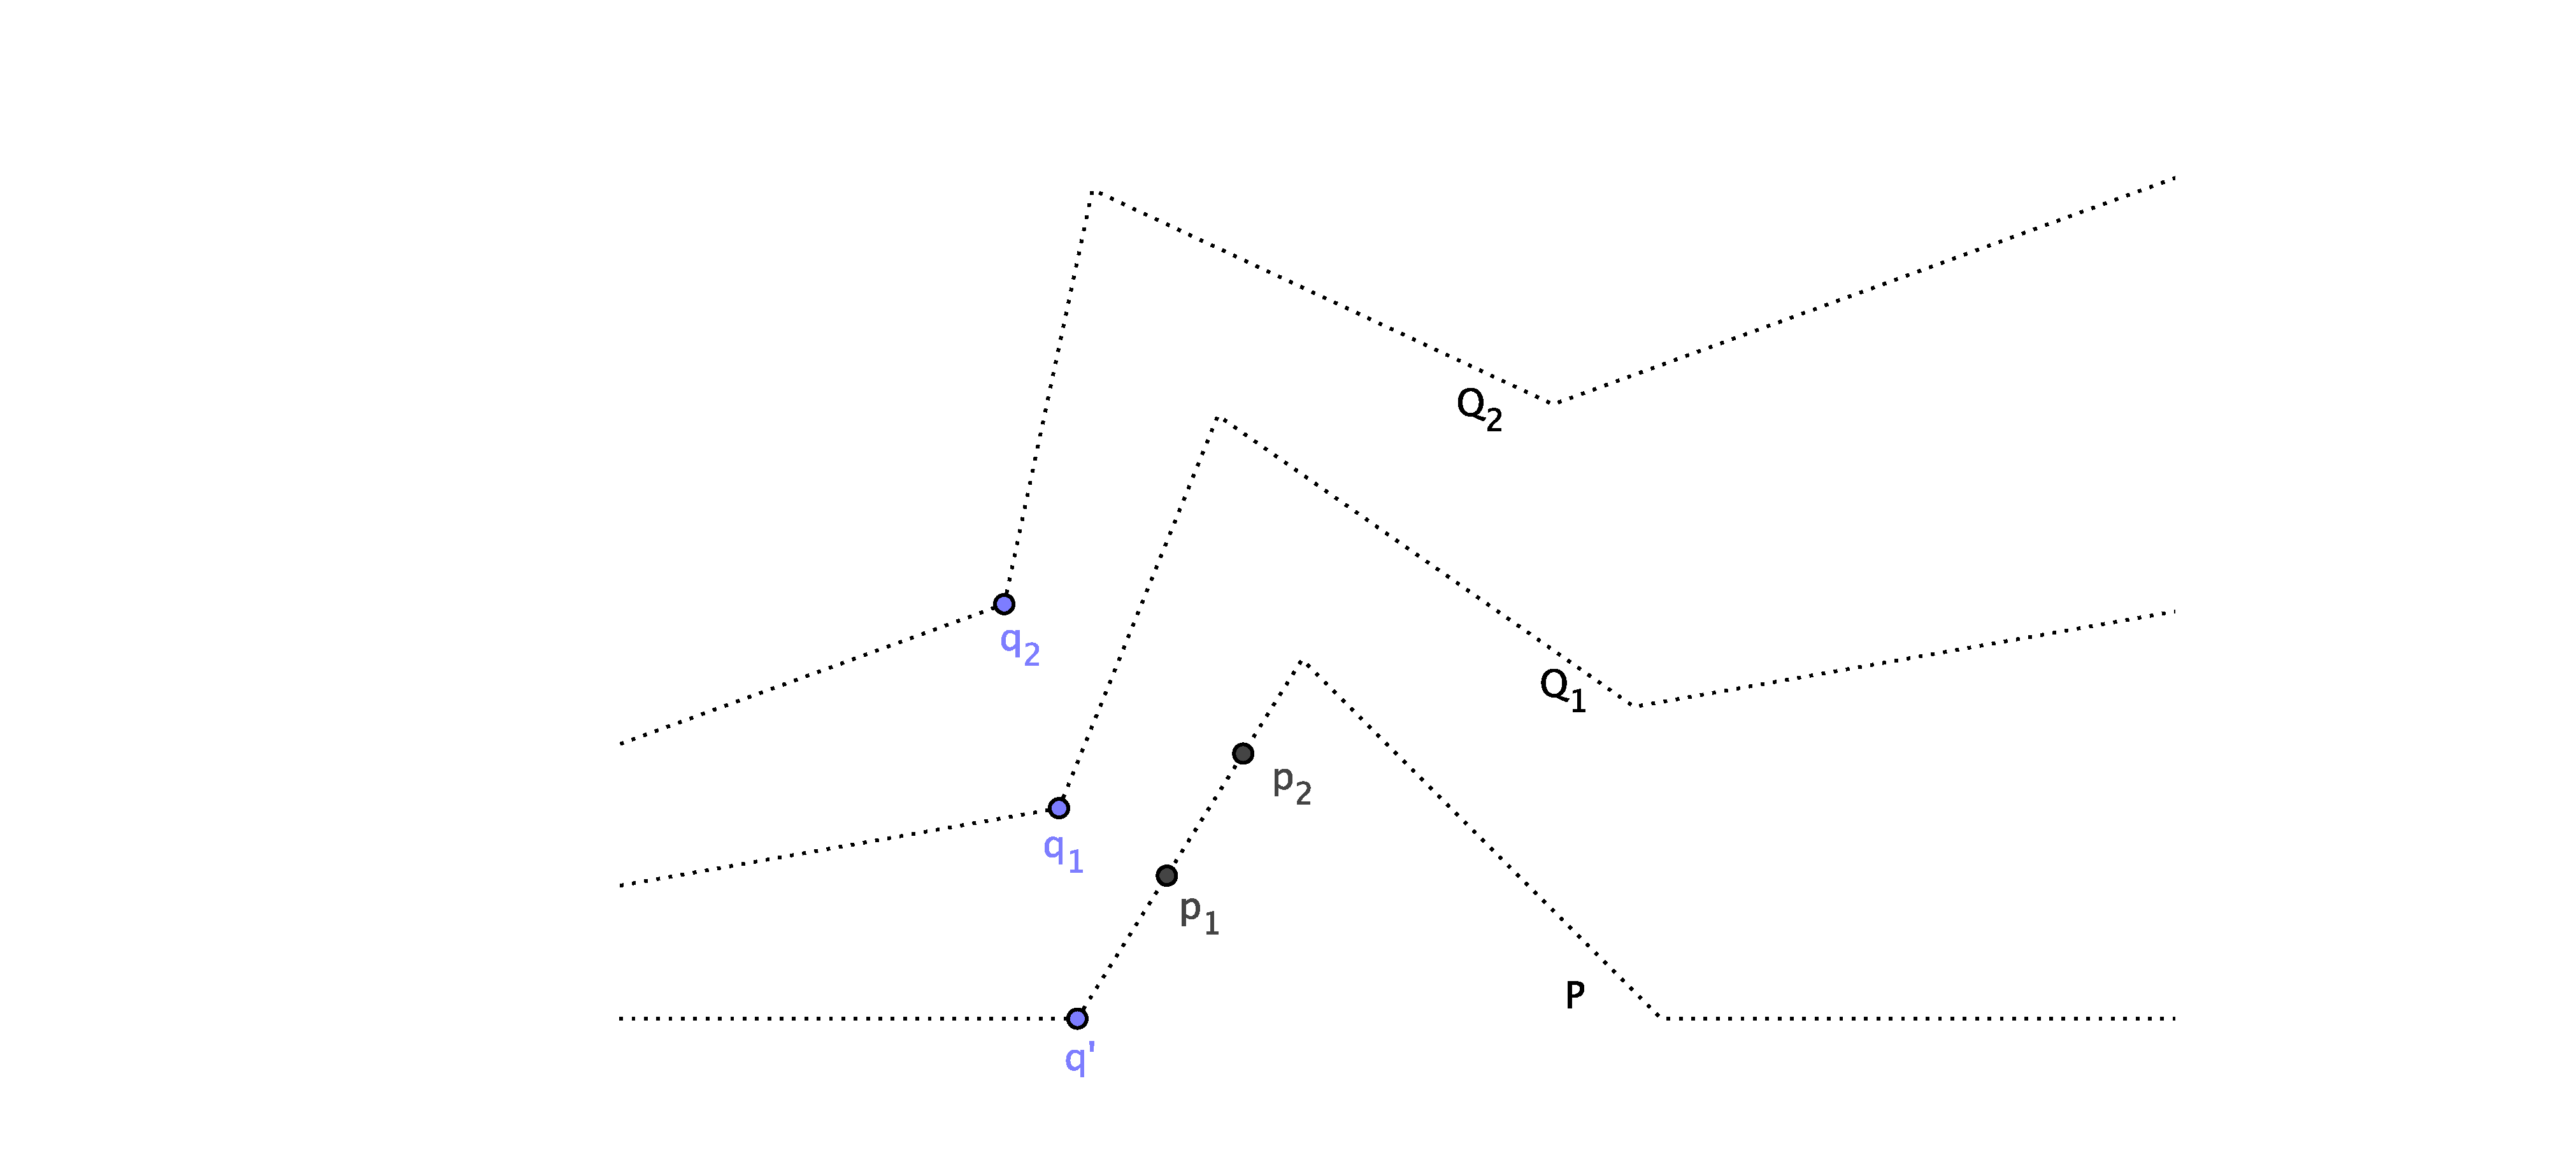
\includegraphics[width=.5\textwidth]{fig/icp_true_approx_cor.pdf}
\caption{Single point at two \gls{icp} iterations}
\label{fig:icp_true_approx_cor}
\end{wrapfigure}
The figure shows a fixed point cloud $P$, and a loose point cloud $Q$ at two different alignments, $Q_1$ being aligned more accurately than $Q_2$. $q_2, q_1, q'$ represent the same position, in the coordinate systems of the three point clouds. $q \in Q$, but in general $q' \notin P$ except when $Q$ and $P$ have exactly the same constellation.
$p_1, p_2 \in P$ are the correspondence points chosen for $q_1$ and $q_2$ by the closest point criterion.

Hypothesis (1) translates into $d(q_1, q') < d(q_2, q') \Rightarrow d(p_1, q') < d(p_2, q')$. If the point clouds consisted only of the line $\bar{q' p_1}$ this would be true from the triangle similarity. Clearly $\lim_{q \rightarrow q'} d(p, q) = 0$. But the convergence is generally not monotonous. For example if $q$ were to come in from another angle, $p$ could oscillate between the closest points from the two line segments adjacent to $q'$.

The error minimization step pulls all $q_i$ closer to $p_i$. Because $\{ p_i \}$ and $\{ q_i \}$ have different constellations, they cannot be made to coincide, but $d(p_i, q_i)$ will get smaller in the least squares sense. \footnote{If it were to get larger, then $\matr{I}$ would be a better transformation estimation than the one found by least squares minimization.} This shows that $d(q_1, p_2) < d(q_2, p_2)$. $p_1$ is the closest point to $q_1$ by the closest point criterion, meaning that $q_2$ cannot be closer. Hence $d(q_1, p_1) < d(q_1, p_2) < d(q_2, p_2)$. This proves the convergence of the \gls{icp} algorithm with the closest point criterion.

For hypothesis (2) to be satisfied, it must additionally be true that $d(q', p_1) < d(q', q_2)$. When this is not true, the algorithm can converge towards a local minimum.

In \cite{Liu2008} additional geometric properties of the closest point criterion are identified, which justify its use for point set registration and other application, and show that the correspondences are of ``high relative'' quality.



\subsubsection{Local minima}
\gls{icp} minimizes an error function $e_{\matr{M_c}} : \matr{M} \mapsto \mathbb{R}$ taking as input a rigid transformation. The function $e_{\matr{M_c}}$ is different at each iteration, and depends on current correspondences. $\matr{M_c}$ denotes the transformation estimation for this iteration, based on which the correspondences were taken.

One can define a ``global'' error function $e(\matr{M}) = e_\matr{M}(\matr{M})$. It is non-continuous because different correspondence pairs get chosen as $\matr{M}$ changes, and it can not directly be minimized. The global minimum of $e$ represents the sought after optimal transformation. $e$ can be though of as a best possible error function \gls{icp} could encounter during the iterations. Since the correspondences change only at discrete locations, $e$ is equal to one of the ``local'' error functions $e_{\matr{M_c}}$ in the neighborhood of an input $\matr{M}$.

Each local error function $e_{\matr{M_c}}$ (for fixed $\matr{M_c}$) generally has one global minimum and no local minima, unless there is some symmetry in the point constellation. At each iteration $\matr{M}$ is moved to this minimum. For each $e_{\matr{M_c}}$ the global minima will be different because the correspondences are not correct, and each of those global minima forms a local minimum in the global error function $e$.

To summarize:
\begin{figure}[H]
\begin{tabular}{r|l|l}
Error function & global error function $e$ & local error function $e_{\matr{M_c}}$ \\ \hline
Correspondences & depend on input & fixed, depending on $\matr{M_c}$ \\
Global minimum & optimal transformation & transformation estimation \\
Local minima & global minimum of $e_{\matr{M_c}}$, incorrect convergence & generally none \\
Minimization & no direct solution & least squares or other \\
Continuous & no & yes \\
Computation & expensive, need to compute correspondences & cheap
\end{tabular}
\end{figure}

Figure \ref{fig:icp_glob_err_example} is an example of a global error function $e$. The Y axis indicates the value $e(\matr{M})$, the X axis is an interpolation between two randomly chosen points in the $6$-dimensional space of rigid transformations. Visualization of error metrics will be described in more detail in section \ref{sec:err_vis} of the next chapter. The point clouds $P$ and $Q$ used here are two different, coarsely aligned scans of the same object. It can be seen that that the optimal transformation is likely in the region shown at $x \approx -0.2$. But local minima appear farther off, as well as some smaller ones due to discontinuities.

It is possible for \gls{icp} to converge towards one of the local minima at $e(\matr{M}_{\text{lmin}})$. All the local error functions $e_\matr{M}_{\text{near lmin}}$ in which take effect in the neighborhood of $\matr{M}_{\text{lmin}}$, will still their global minimum near $\matr{M}_{\text{lmin}}$.

\begin{figure}[h]
\centering
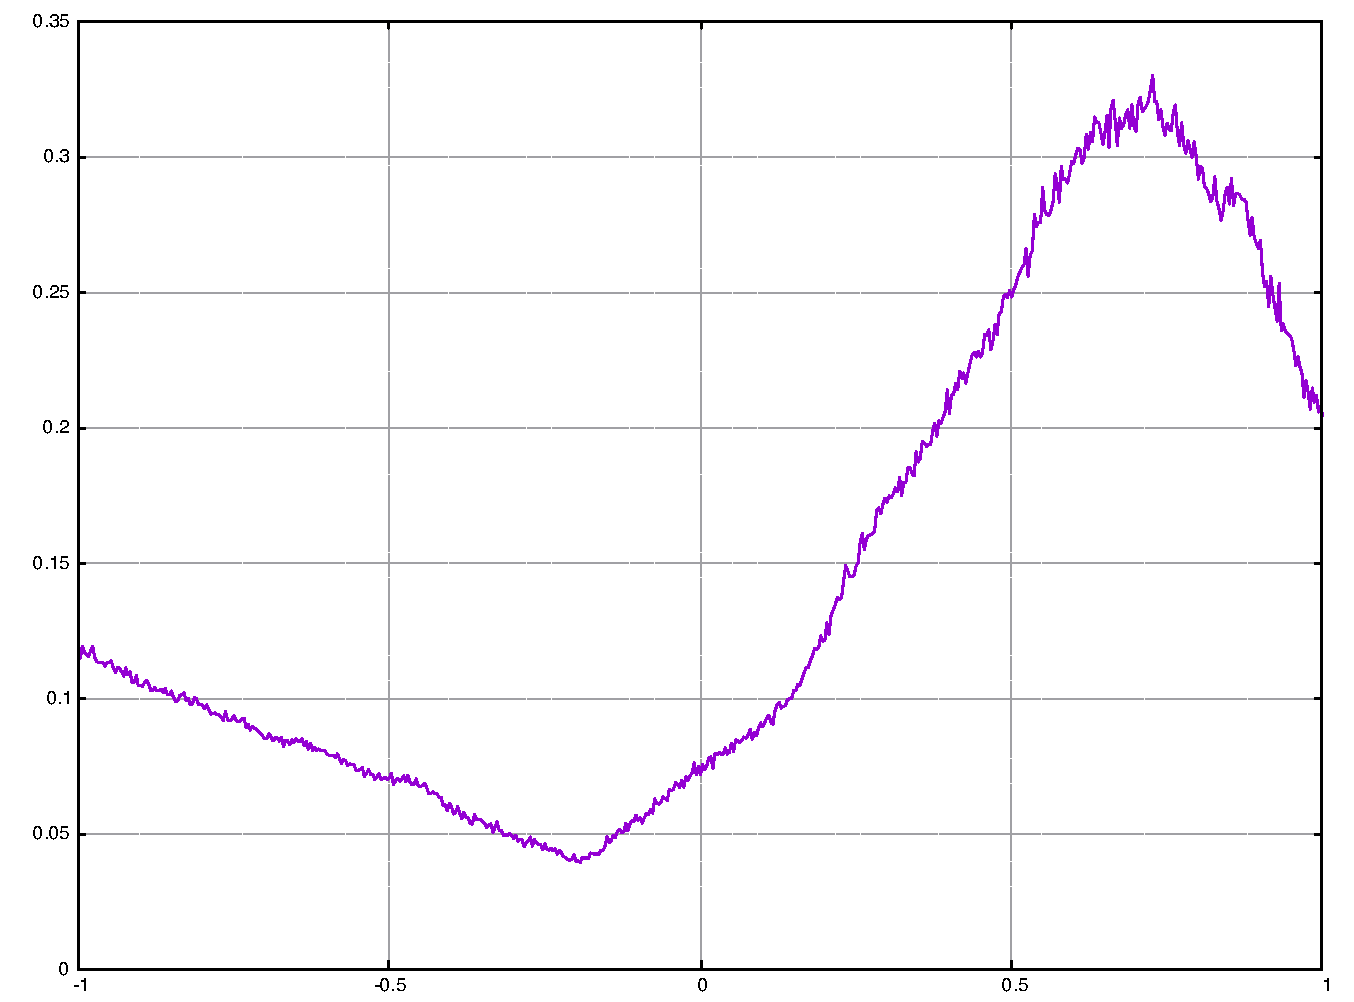
\includegraphics[width=.4\textwidth]{fig/icp_glob_err_example.pdf}
\caption{Example of global error function $e(\matr{M})$ with local minima}
\label{fig:icp_glob_err_example}
\end{figure}

The Go-ICP algorithm, described in \cite{Yang2013} is a globally optimal method based on \gls{icp}, which always converges towards the global minimum of the error metric $e$. It uses the mentioned properties of the error metrics, and implements a branch-and-bound scheme which searches the space of rigid transformations.

Other, simpler techniques to avoid convergence towards a local minimum, involve injecting some random noise into the estimated transformation at each iteration. The amount of noise decreases with the number of iterations. In a physical analogy, this makes $\matr{M}$ ``jump'' out of the small holes seen on the curve in figure \ref{fig:icp_glob_err_example}, and encourage it to fall onto the global minimum.


\subsubsection{Multi-view ICP}
It is also possible to extend \gls{icp} to multi-view instead of pairwise registration. \cite{Told2010} presents an algorithm within the ICP framework, where the error metric and correspondence finding steps are modified in order to align $k$ point clouds simultaneously.

For the correspondences, instead of pairs of closest points, $k$-tuples of \emph{mutually nearest neighbors} are searched. Each ordered pair $(p, q)$ of two points within a tuple must be such that $p$ is the closest point to $q$. 

For the error minimization, \emph{generalized Procrustes analysis} (GPA) is applied, as described before in section \ref{sec:procrustes}, in order to find the rigid transformations $\matr{M}_i$. At each iteration of \gls{icp}, the GPA target $\matr{K}$ is initialized to the centroids of the correspondence tuples, and then the Procrustes algorithm is run.


\subsubsection{Iterative Dual Correspondences}
\cite{Lu1997} describes the \emph{iterative dual correspondences} algorithm, an variant of \gls{icp} in two-dimensions in which two sets of correspondences are computed at each iteration: One using the closest point criterion, and the second using the ``matching range point rule'': In polar coordinates, the difference between radii is minimized and the difference in angles constrained to a small interval.

For the error metric the closest point correspondences are used for the translation estimation, while the rotational estimation is computed using the matching range point rule correspondences.

This method was shown to be more robust than standard \gls{icp} when the error in the initial pose is large. \cite{Magn2013}


\subsubsection{Probabilistic Iterative Correspondence}
This method is described in \cite{Mont2005}. It incorporates information from scanner errors and the uncertainty of the initial pose estimate, by modeling the points as random variables taken from a Gaussian distribution. Generalized ICP is a similar approach. It is described in more detail in the next section.


\subsubsection{Sparse ICP}
The least \emph{squares} error metric used by \gls{icp} poses the problem that outliers and wrong correspondences, which have greater distances than good correspondences, get an over-proportionally high weight in the error metric. This makes \gls{icp} sensitive to noise in the input point clouds.

Sparse ICP, described in \cite{Boua2013}, is a variant which instead minimizes an error metric $\sum_i \| p_i - \matr{M} \, q_i \|^p$ with $p < 1$. Geometrically this still measures the Euclidian distance, but that number is put to a power other than $2$, giving correspondences with lower distance a higher weight.

The error metric is \emph{sparse} in the sense that the correspondences get implicitly classified into outliers and inliers, because $\|d\|^p \approx 0$ for inliers and $\|d\|^p \approx 1$ for outliers.

The error minimization is done with the \emph{alternating direction method of multipliers}, which essentially translates it into two least squares problems.



\subsection{Generalized ICP}
Conceptually, the difference between point-to-point \gls{icp} and point-to-plane \gls{icp} is that in the point-to-plane variant, the position of a point on a surface has no impact on the error metric and minimization. This is useful because the point clouds represent solid surfaces approximated using a discrete set of points, and the goal of a registration algorithm is to align those surfaces, and not the points that represent it. The registration algorithm should be agnostic to the distribution of points on a surface.

\emph{Generalized ICP}, first described in \cite{Sega2009}, is a generalization that covers both of these variants. Each point is replaced by a three-dimensional gaussian probability field that models the uncertainty of its position on the surface and orthogonal to the surface. A new error metric formula to minimize is deduced that includes covariance matrices for the two points' distributions. The other components of the ICP framework are not changed, and in particular, points correspondences are still established using the closest point criterion.

Let $p \in P$ and $q \in Q$ be the points from the two point clouds to register, and let $(p_i, q_i)$ represent pairs deemed to be corresponding points by the closest point criterion or other. The model assumes the existence of underlying sets of unknown points $\{ p'_i \}$ and $\{ q'_i \}$ which are such that the correspondences are perfectly correct. That is, $\foreach i : p'_i = \matr{M} \, q'_i$. The points $p_i$ and $q_i$ on which the registration is performed are redefined to be random variables generated from $p'_i$ and $q'_i$, taken from a normal probability distribution.
\begin{equation}
p_i \sim \mathcal{N}(p'_i, \matr{C}^{P}_i)
\hspace{7mm} \text{and} \hspace{7mm}
q_i \sim \mathcal{N}(q'_i, \matr{C}^{Q}_i)
\end{equation}
The expression $\mathcal{N}(p'_i, \matr{C}^{P}_i)$ represents a three-dimensional multivariate normal (gaussian) distribution, with $p'_i$ as mean and with covariance matrix $\matr{C}^{P}_i$. The mean $p'_i$ is unknown, and $\matr{C}^{P}_i$ (and $\matr{C}^{Q}_i$) are attributes which get associated to each point beforehand.

This models both (1) the error in the points $p'_i$ and $q'_i$ which makes them deviate from the underlying surface, and (2) the imprecision of the correspondences due to the different point dispersions on $P$ and $Q$.

Let $d_{i,\matr{M}}$ be the distance between $p_i$ and $q_i$ with estimated transformation $\matr{M}$.
\begin{equation}
d_{i,\matr{M}} = p'_i - \matr{M} \, q'_i
\end{equation}

Because $p_i$ and $q_i$ are assumed to have been taken from two independent normal distributions, their distance $d(p_i, q_i)$ is also a random variable with a normal distribution that can be expressed in terms of $C^{P}_i$, $C^{Q}_i$ and the unknown true transformation $\math{M}$:
\begin{equation}
d_{i,\matr{M}} \sim \mathcal{N}(0, \matr{C}^{P}_i + \matr{M} \, \matr{C}^{Q}_i \, \transpose{\matr{M}})
\end{equation}

Using maximal likelihood estimation, $\hat{\matr{M}}$ can be estimated:
\begin{equation} \label{eq:gen_icp_err}
\begin{align}
\hat{\matr{M}} &= \argmax_{\matr{M}} \prod_{i} p(d_{i,\matr{M}}) \\
&= \argmax_{\matr{M}} \sum_{i} \log(p(d_{i,\matr{M}})) \\
&= \argmin_{\matr{M}} \left[ \transpose{d_{i,\matr{M}}} \, (\matr{C}^{P}_i + \matr{M} \, \matr{C}^{Q}_i \, \transpose{\matr{M}})^{-1} \, d_{i,\matr{M}} \right]
\end{align}
\end{equation}
This is the error metric which is minimized by the generalized ICP algorithm.

\subsubsection{Covariance matrices}
When $\matr{C}^{P}_i = \matr{I}$ and  $\matr{C}^{Q}_i = 0$, the error metric simplifies to the point-to-point error metric. The three diagonal components of $\matr{C}^{P}_i$ represent the variances of the position of $p_i$ relative to $p'_i$, along the X-, Y- or Z-axis. These axis in world space are meaningless in the context of the local neighborhood of points, and instead the coordinate system is set such that one axis is the normal vector of the point. These normal vectors need to have been computed beforehand. So
\begin{equation}
\matr{C}^{P}_i = \matr{R}_{i} \, \left( \begin{matrix}
x & 0 & 0 \\
0 & y & 0 \\
0 & 0 & z
\end{matrix} \right) \, \transpose{\matr{R}_{i}}
\end{equation}
Where $\matr{R}_i$ is a rotation matrix which rotates the surface normal vector $\vec{n}$ of point $p_i$ to the X axis. Now $x$ is set to a low value because a deviation along the axis of the normal vector corresponds to a deviation from the underlying surface and can be considered a scanner error. $y$ and $z$ represent a deviation along the local tangent plane of the surface, and is set to a larger value because a greater deviation is expected due to different point dispersions. The remaining components are set to $0$ since there is no covariance on the differences in two directions. When $x = 0$ and $y,z \rightarrow \infty$, the formula \ref{eq:gen_icp_err} becomes the point-to-plane error metric. $\matr{C}^{Q}_i$ is constructed in an equivalent way.


\subsection{Normal Distributions Transform}
The \gls{ndt} algorithm is an approach which converts the point clouds into a piecewise continuous representation, called the \emph{normal distributions transform}, and then registers them using continuous optimization. It is first described by \cite{Bibe2003} in the context of robotics, for two-dimensional point clouds representing a map of a mobile robots's environment. Starting with an initial alignment taken from movement sensors on the robot, the algorithm performs fine registration of the map with a model point cloud in an efficient way.

Both two-dimensionals point cloud $P$ and $Q$ are split into a grid of regular square cells. For each cell a gaussian is calculated which best represents the distribution of points in that cell. Let $n$ be the number of points in one cell, and let $\{ p_i \}$ be the set of those $n$ points.

The gaussian is a two-dimensional multivariate normal distribution. Its mean $\vec{\mu}$ and its $2 \times 2$ covariance matrix $\matr{C}$ are calculated from the point in the cell:
\begin{equation}
\vec{\mu} = \frac{1}{n} \sum_{i=1}^{n} \vec{p_i}
\hspace{7mm} \text{and} \hspace{7mm}
\matr{C} = \frac{1}{n - 1} \sum_{i=1}^{n} (\vec{p_i} - \vec{\mu}) \transpose{(\vec{p_i} - \vec{\mu})}
\end{equation}
Let $p(\vec{x})$ be the probability density function of this gaussian. Now the surface integral of $p$ over an area $\mathcal{A}$, multiplied by $n$, gives an expected value of the number of points in that area. $p(\vec{x})$ represents the marginal probability that there is a point at position $\vec{x}$. Because of this $\sum_i p(\vec{x_i})$ is maximal when all $x_i$ are points from $P$.

The normal distribution transform consists the two-dimensional array of these gaussians, for each cell of the grid. Computationally $6$ real values are stored per cell ($\vec{mu}$ and $\matr{C}$). The registration will be performed only using those values, without looking at the underlying points. For the fixed point cloud $P$, it is sufficient to store only the normal distribution transform.

The algorithm proceeds in the following steps:
\begin{enumerate}
\item The \gls{ndt} for the fixed point cloud $P$ is created.
\item The transformation parameters $T = (t_x, t_y, \phi)$, which are going align $Q$ to $P$, are initialized to some first estimation.
\item The loose point cloud $Q$ is transformed according to $T$.
\item For each point $q_i \in Q$, the cell $c_j$ from the \gls{ndt} of $P$ in which it falls is determined, which is trivial because it is a regular square grid.
\item The estimation of $T$ is improved by maximizing the \emph{score} $\sum_{i=1}^{N(Q)} p_{c_j}(\vec{q_i})$. Here $p_{c_i}$ is the probability density function of the gaussian in the cell $c_i$ from the \gls{ndt} of $P$. As stated before it is maximal when $\{ q_i \}$ and $\{ p_i \}$ coincide. The maximization of the (continuous) score function is done using the multi-dimensional Newton's method.
\item Repeat from step 2, until $T$ stabilizes.
\end{enumerate}

\cite{Dold2007} describes a simple way to extend the \gls{ndt} algorithm to three dimensions, but still for two-dimensional transformation parameters: The point clouds is split into multiple 2D cross-sections, for example on different height layers. Then the sums of the score functions of the different layers are maximized.

A real three-dimensional form of \gls{ndt} is presented in \cite{Magn2007} and further elaborated in \cite{Magn2013}. Here the cells are cubic 3D subspaces, and a 3D rigid transformation is computed. The complexities of 3D rotation complicate this problem. In addition to this, a fixed discretisation, where the space is divided into a regular grid of same sized cubes is usually not appropriate: Since the point cloud is an embedding of two-dimensional surfaces in three-dimensional space, the three-dimensional density is not uniform and sparsely distributed. So smaller cube sizes are required in some parts, and not in others. The articles suggest instead an Octree discretisation where different sized overlapping cubes forming an Octree are used, or alternatively an iterative discretisation. Here cube sizes are reduced at each iteration as the algorithm progresses and the transformation estimation gets closer to convergence.

\cite{Magn2013} also addresses irregularities due to the discontinuities at the cell boundaries using an interpolation method, and the inclusion of color data from the point attributes into the \gls{ndt} score maximization.


\subsection{4-Points Congruent Sets}
The \gls{4pcs} algorithm, a completely different approach for fine point cloud registration, is presented in \cite{Aige2008}. An improved version called Super-4PCS is described in \cite{Mell2014}. It is based on a \gls{ransac} scheme, and is essentially an improvement to the basic method described before in section \ref{sec:ransac_pc} which reduces its complexity and convergence speed.

The algorithm proceeds according to the following steps:
\begin{enumerate}
\item Instead of choosing three point pairs as sample, \gls{4pcs} starts by randomly choosing a quadruplet\footnote{A quadruplet of points is called a ``4-points'' in the article.} of approximatively coplanar points from the fixed point cloud $P$. This sample $S$ will be called the \emph{base}.

\item Now the set $U$ of quadruplets of points from $Q$, which are \emph{congruent} to the base $S$ is computed. Congruent means that $S$ and $u_i \in U$ are (approximatively) related by a rigid transformation $\matr{M}_i$.

\item For each $u_i$, a consensus set $S^{*}_i \in Q$ is computed which consists of the points $q \in Q$ such that
\begin{equation*}
\min_{p \in P} \| p - \matr{M}_i q \|
\end{equation*}
is below some threshold distance. These are the points $q \in Q$ that would get moved close to the point cloud $P$ by the transformation $\matr{M_i}$.

When $\matr{M_i}$ is accurate, $S^{*}_i$ will include all the points from $Q$ that have a close corresponding point in $P$. If the planes spanned by $S$ and $u_i$ are approximatively parallel in $P$ and in $Q$ (in their respective coordinate systems), then a good estimate for $\matr{M_i}$ was found.

\item The consensus set $S^{*}$ is then formed by taking the $S^{*}_i$ which contains the largest number of points. Its corresponding $\matr{M_i}$ becomes a candidate for the final transformation estimation. It is the best transformation that can be found using $S$ as \emph{base}. 

\item The algorithm is repeated several times, each time with a different, randomly chosen base. At the end the best candidate for the transformation estimation, for which $\| S^{*} \|$ was the largest, is retained.
\end{enumerate}


Because of the \gls{ransac}-based approach of choosing inlier points, \gls{4pcs} is robust to noise. It also does not need any initial alignment of $P$ and $Q$.


\subsubsection{Search of congruent quadruplets}
The fundamental operation of the \gls{4pcs} operation is its second step, in which the set of all quadruples that are congruent to $S$ is computed. A naive implementation would consider all $|Q|^4$ sets of four points from $Q$, and then check if they are coplanar, and if they are congruent to $S$.

Because the $4$ points in $S = (p_1, p_2, p_3, p_4)$ are coplanar, they necessarily contain two pairs of points that form intersecting lines. Without loss of generality, let $p_1 p_2$ and $p_3 p_4$ be those lines, and $i_p$ their intersection point.

It can be shown that the numbers
\begin{equation} \label{eq:4pcs_inv}
r_1 = \frac{\| p_1 - i_p \|}{\| p_1 - p_2 \|}
\hspace{7mm} \text{and} \hspace{7mm}
r_2 = \frac{\| p_3 - i_p \|}{\| p_3 - p_4 \|}
\end{equation}
are invariant with respect to an affine transformation of the four points, and that they always change when a non-affine transformation is applied to them. As a consequence, $r_1$ and $r_2$ must have the same values for the searched congruent quadruplets $u_i = (q_1, q_2, q_3, q_4)$ taken from $Q$.

The algorithm now iterates through $Q$ and considers all ordered pairs $q_i, q_j$ of points from $Q$, and makes the hypothesis that they belong into one of the searched quadruplets $u_i$ and that they form one of its two intersecting lines. If that is true there are two possible positions for the position of their intersection point:
\begin{equation}
i_{q,1} = q_i + r_1 (q_j - q_i)
\hspace{7mm} \text{or} \hspace{7mm}
i_{q,2} = q_i + r_2 (q_j - q_i)
\end{equation}

When during the iterations two pairs of points $(q_i, q_j), (q'_i, q'_j)$ are such that $i_{q,1} = i'_{q,2}$, it is likely that $u_i = (q_i, q_j, q'_i, q'_j)$ is one of the congruent quadruplets.

This is a necessary, but not a sufficient condition: The values $r_1$ and $r_2$ are invariant for \emph{affine} transformations, but for $S$ and $u_i$ to be congruent quadruplets they must be related by a \emph{rigid} transformation. Therefore a filtering stage is added to remove the wrong quadruplets. 


\subsubsection{Choice of base}
To choose a base $S$, the algorithm first randomly takes three points of $P$. They are always coplanar. Points with greater distances are preferred. Then the fourth point is chosen such that the quadruple is coplanar.
